%% amssamp1.tex is nearly identical to amssamp2.tex, except
%% that amssamp2.tex uses the [twocol] option to produce
%% two-column text.

%\documentclass{ametsoc}
\documentclass[twocol]{ametsoc}
\journal{jtech}

%\usepackage{amsmath}
%\usepackage{hyperref}
\usepackage{color}

\usepackage{graphicx}
\graphicspath{{./fig/}}

%%%%%%%%%%%%%%%%%%%%%%%%%%%%%%%%
%Citations should be of the form ``author year''  not ``author, year''
\bibpunct{(}{)}{;}{a}{}{,}

\title{Turbulence spectral estimates from motion-sensor equipped ADVs on compliant moorings}

\authors{Levi Kilcher\correspondingauthor{National Renewable Energy Laboratory, Golden, Colorado}, Jim Thomson, Samuel Harding and Sven Nylund}

\affiliation{} 

\email{Levi.Kilcher@nrel.gov}

%\extraauthor{Extra Author}
%\extraaffil{Affiliation, City, State/Province, Country}

\graphicspath{{./fig/}}
\newlength{\onewidth}
\setlength{\onewidth}{3.2in}

\newcommand{\note}[1]{\textcolor{blue}{#1}}
\newcommand{\citeneeded}[1]{\textcolor{red}{(NEED CITATION for: #1)}}
\usepackage{defs}

\abstract{
THE ABSTRACT.
}

\begin{document}

\maketitle


\section{Introduction}

% Invented more than twenty years ago, acoustic Doppler velocimeters (ADVs) measure 3-components of velocity by measuring the Doppler shift of an emitted acoustic pulse at 3 

Since their invention more than twenty years ago acoustic Doppler velocimeters (ADVs) have been used to measure turbulent velocities in a wide range of environments. Originally designed to make point-measurements in laboratory flumes and tanks, ADVs have become an increasingly useful tool in the oceanic environment. They have been deployed, for example, on the seafloor to measure fluxes in the oceanic bottom boundary layer, in the surf-zone to measure Reynold's stresses, and from ships on downward protruding masts to measure surface mixing \citep[e.g.]{Lohrmann++1994, Voulgaris+Trowbridge1998, Kim++2000, Trowbridge+Elgar2003, Elgar++2005, Geyer++2008}.

Why is the turbulence spectrum important? -- Captures motion at all scales.
ADCPs 
1) History of ADV use. How are they used? In what turbulence levels? What is their noise-floor? 
1a) How do they compare to other turbulence tools?
Compared to profilers, ADVs are:
  - Lower precision than profilers at high f?
  - Capture low-frequency information.
  - can be fixed in space.
Compared to ADCP, ADVs can capture the turbulence spectrum:

  - Higher precision at high f
  - Higher resolution (down to cm scales)
  - Lower noise

Say something about: we don't have independent measurements of turbulence to validate against, so we use spectra--and our knowledge of their theoretical properties--to gain confidence in the method.

A primary limitation of ADVs is that it has been challenging to place them at mid-depths (i.e. away from the seafloor and the surface). In the oceanic environment they have either been deployed on fixed platforms anchored to the sea-floor, or deployed near the surface from a ship.  Until now, there has been no method for deploying these instruments at mid-water depths, or near the surface without a ship.  This work describes a new approach for measuring turbulence spectra from ADVs mounted on moorings. Until recently this approach has been limited by the fact that mooring motion contaminates the velocity measurements.  The frequency and amplitude of this contamination will depend on the characteristics of the mooring and of the turbulent environment in which it is deployed. In most cases mooring motion will--over some range of frequencies--be similar to or greater than the turbulence velocities one would like to measure. This `motion contamination' reduces usefulness of the ADV measurements. 

Over the last decade, the cost of inertial motion sensors (IMUs)

However, this being said,  In many cases the motion of the mooring Depending Because When the mooring (and ADV head) moves with the flow the measured velocity will be reduced, and when it moves against the flow it will enhance the it. is often equal to the turbulent velocities one would like to measure. contaminates the velocity measurements  equipped with 

In energetic environments ADVs provide 

In energetic environments, where turbulence levels ADVs provide are Throughout 

Velocity measurements have been made from 

As flexible and useful as these instruments are, one limitation 
% boundary-layer studies. 

are useful tools for making point-measurements of water velocity in labarotory and field environments. 
robust and versatile tools 

  ADV velocity measurements from compliant moorings will be contaminated by mooring motion. When an inertial motion unit (IMU, also known as a magnetic, angular rate, gravity or MARG sensor) is rigidly attached to, and tightly synchronized with, acoustic Doppler velocimeter (ADV) measurements the IMU's orientation and motion measurements can be used to reduce motion contamination.  Microstrain IMU on-board the Nortek Vector is equipped with a 3-axis accelerometer, a 3-axis rotation-rate sensor, and a 3-axis magnetometer.  The Microstrain samples these signals at 1000Hz and performs integration and Kalman filtering operations to produce stable estimates of it's orientation, change in velocity, and change in rotation-rate.  and  can be configured to output estimates of,

\section{Measurements}
\label{sec:meas}

This work is focused on measuring turbulence spectra from moored ADVs that are equipped with inertial motion sensors (IMU). The ADVs utilized for these measurements were all equipped with Microstrain 3DM-GX3-25 IMU sensors that captured all 6 components of the ADV motion (3 components of angular rotation and 3 components of linear acceleration), as well the orientation of the ADV pressure-case. The sampling of the motion sensor is tightly synchronized with the ADV measurements. The IMU measures its motion at 1kHz and uses internal signal integration (Kalman filtering) to output the motion signals at the same sample rate as the ADV's velocity measurements. This reduces aliasing of the IMU's motion measurements above the ADV's sample-rate \cite{3DM-GX3_coning_sculling}.

\subsection{Measurements}

This work utilizes data from two distinct mooring systems to demonstrate the advantages and limitations of each platform. Both mooring systems were deployed in Admiralty Inlet, Washington, approximately 500 meters (m) WSW of Admiralty Head--Fort Casey State Park--in 60 m of water at latitude 48.153 north and longitude 122.687 west (Figure \ref{fig:map}). Admiralty inlet possesses a large semi-diurnal tidal energy flux as it is the largest waterway connecting Puget Sound to the Strait of Juan de Fuca. The site is approximately 6 kilometers (km) east of Port Townsend, and 1 km north of the Port Townsend -- Coupeville ferry route.

\begin{figure}[t]
  \centering
  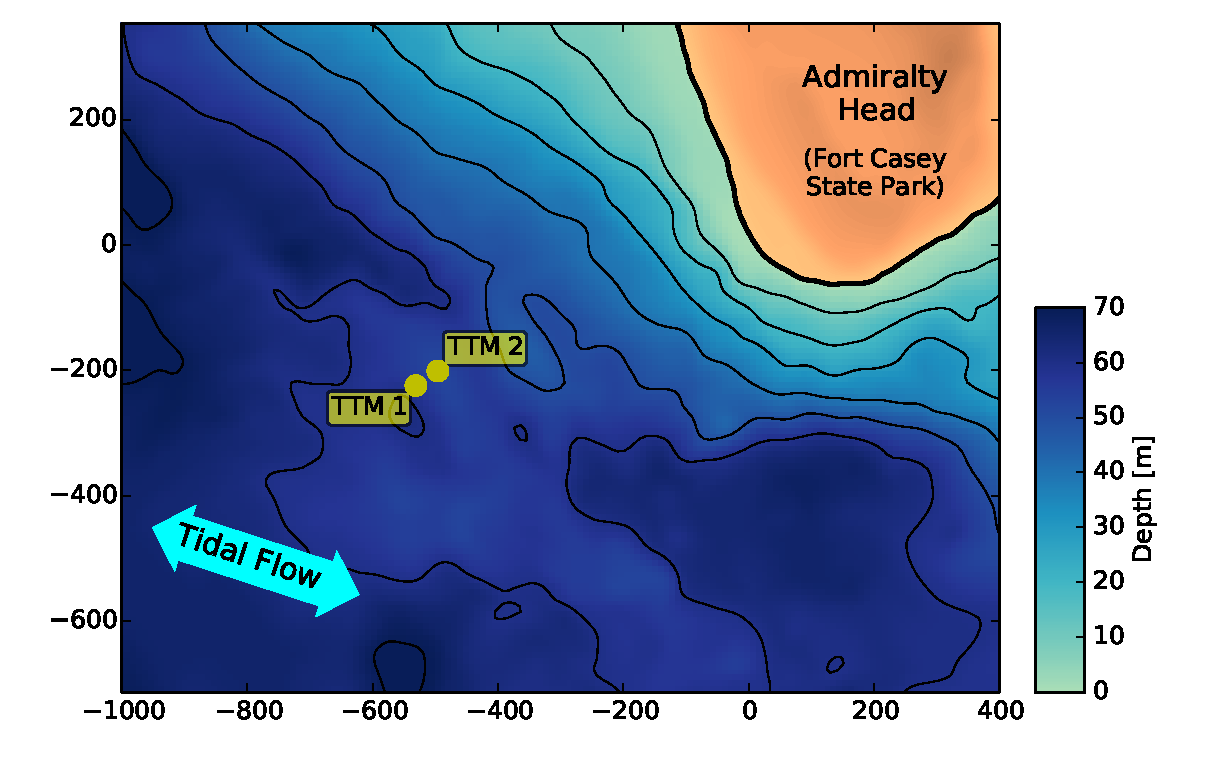
\includegraphics[width=3.4in]{map02}
  \caption{Bathymetry of Admiralty Inlet at Admiralty Head.}
  \label{fig:map}
\end{figure}

\subsubsection{Tidal Turbulence Mooring (TTM)}

The `Tidal Turbulence Mooring' (TTM) is a simple mooring system with a `strongback fin' suspended between a clump-weight anchor weighing 1200 kilograms (kg, dry) and a 0.93 m-diameter spherical steel buoy with a buoyancy of 320 kg \note{will I catch flak for using `kg' for `buoyancy'?}. The ADV pressure cases were clamped to one side of a `strongback' fin and the ADV sensor head was positioned 10cm in front of the fin's leading edge (Figure \ref{fig:ttm:diagram}). The leading edge of the fin is fastened inline with the mooring line. This configuration  was designed to work similar to a weather-vane, such that the drag on the fin held the ADV head upstream of the mooring components.  This work utilizes data from two TTM deployments. 

The first was in June, 2012\note{... deployment dates, lat/lon.} Two ADVs were clamped to the fin such that the $z$-axis of the ADVs were parallel with the leading edge of the strongback. Only one of these ADVs was equipped with an IMU, the other was a traditional Nortek Vector. This TTM was equipped with an upward-looking acoustic Doppler profiler on the mooring anchor.

Periods of time during which this mooring interfered with a beam of the Doppler profiler were identified by inspection of the profiler's acoustic amplitude signal. Periods during which one beam of the profiler had $>5\%$ higher acoustic amplitude than the other beams were flagged as `contaminated' and excluded from averaging.  5-minute averages in which more than 50\% of the data was contaminated in this way are not shown.

The second TTM deployment was in June 2014\note{... deployment dates, lat/lon.} Two ADVs were mounted on this TTM. In this case, the ADVs were inclined at an angle of 18$^\circ$ to the leading edge of the fin to account for mooring blow-down during strong currents (Figure \ref{fig:ttm:photo}). The Contrary to the June 2012 deployment, during this deployment the ADV pressure cases were rotated such that the axis of the cylinder is parallel to the stream-wise flow when the mooring blows down at an angle of 18$^\circ$. This change reduces vibrational motion believed to be associated with vortex shedding from the ADV pressure cases when they are oriented cross-wise to the flow (as in the June 2012 deployment).

\begin{figure}[t]
  \centering
  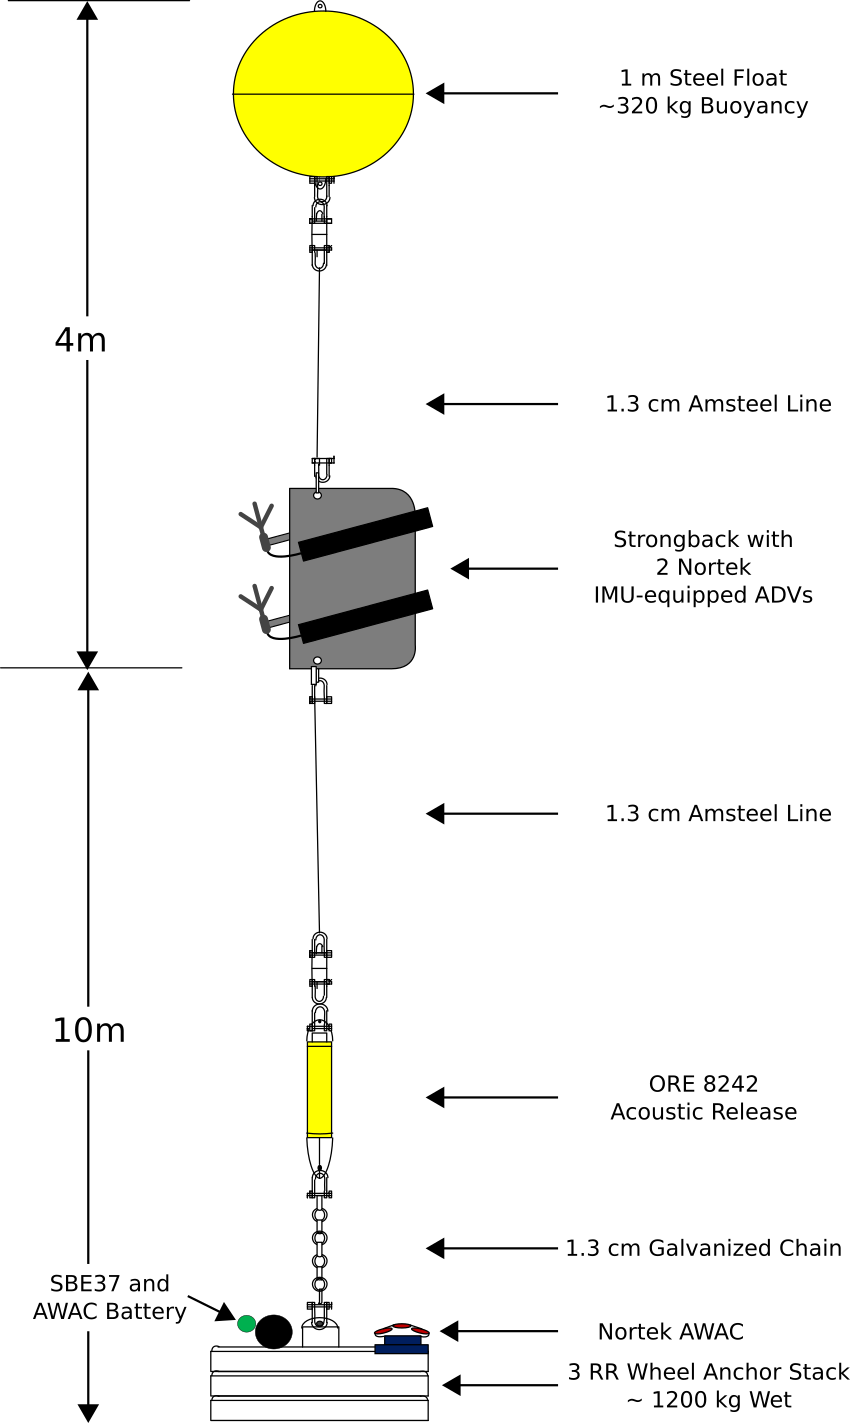
\includegraphics[width=2.4in]{ttm04b}
  \caption{Schematic diagram of the TTM, not to scale.}
  \label{fig:ttm:diagram}
\end{figure}

\begin{figure}[t]
  \centering
  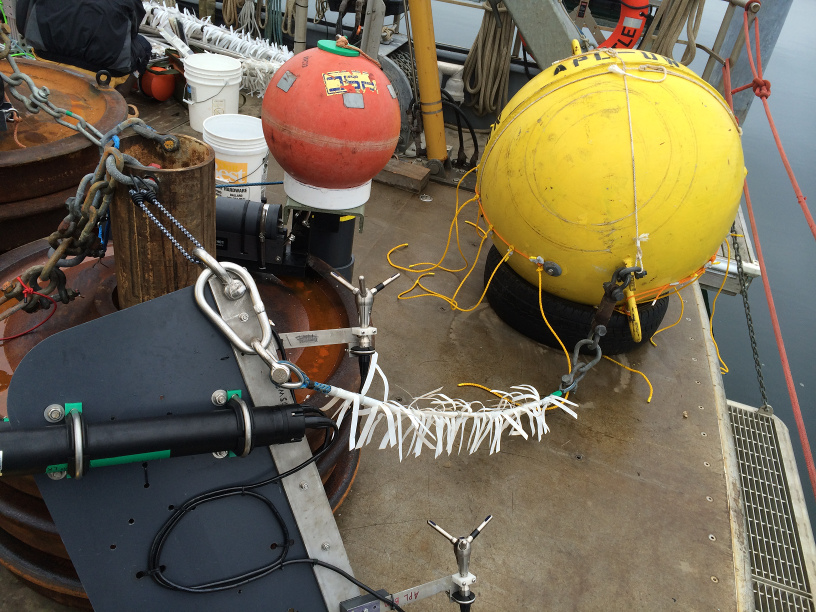
\includegraphics[width=2.6in]{TTM_image01}  
  \caption{TTM components on the deck of the R/V Jack Robertson. The TTM includes two ADVs, with pressure-cases mounted on opposite sides of the fin. The anchor stack includes a pop-up buoy for retrieval. }
  \label{fig:ttm:photo}
\end{figure}

\subsubsection{StableMoor}

The second mooring system was a cylindrical syntactic foam buoy (manufacturer: Deep Water Buoyancy) that was anchored to a clump weight that weighed 2700 lbs (Figure \ref{fig:SM}). The buoy is 3.5 m long and 0.45 m in diameter with a tail ring that is 0.76 m in diameter. 

The StableMoor platform has two primary advantages compared to the TTM. First, it is significantly more massive and hydro-dynamically stable than the TTM, which reduces the frequency of motions of the platform. The other major advantage of the StableMoor platform is that it is capable of supporting an acoustic Doppler profiler that provides an independent measure of the platform's translational motion by bottom-tracking. The disadvantages of the Stable Moor is that its size introduces new challenges in deployment and recovery, and it is significantly more expensive than the TTM system.

The StableMoor weighs 295 kg in air, and has a buoyancy of 185 kg in water. An ADV head was positioned 0.1 m in front of the buoy nose.  The buoy was equipped with a 300 kHz RDI workhorse acoustic Doppler profiler that was pointed downward and configured to measure water velocity below the platform in \note{how many bins?} and measure buoy motion (`bottom tracking') at 1 Hz. 

% \note{is 1 Hz correct? Check xlim of coherence fig!)}
The buoy platform was ballasted to pitch upward a few degrees in zero-flow to avoid `flying downward'. In the presence of an oncoming current the tail fins help to orient it into the flow. The anchor for this buoy is similar to that of the TTM, including an acoustic release so the mooring and anchor can be recovered separately. Additional details, photos, and schematic diagrams of both mooring systems are available in \cite{Harding_MotionPaper}.

\note{Add deployment dates, lat/lon.}

This provides an estimate of low-frequency platform motion, $\ulow$, that is not subject to the 


\begin{figure}[t]
  \centering
  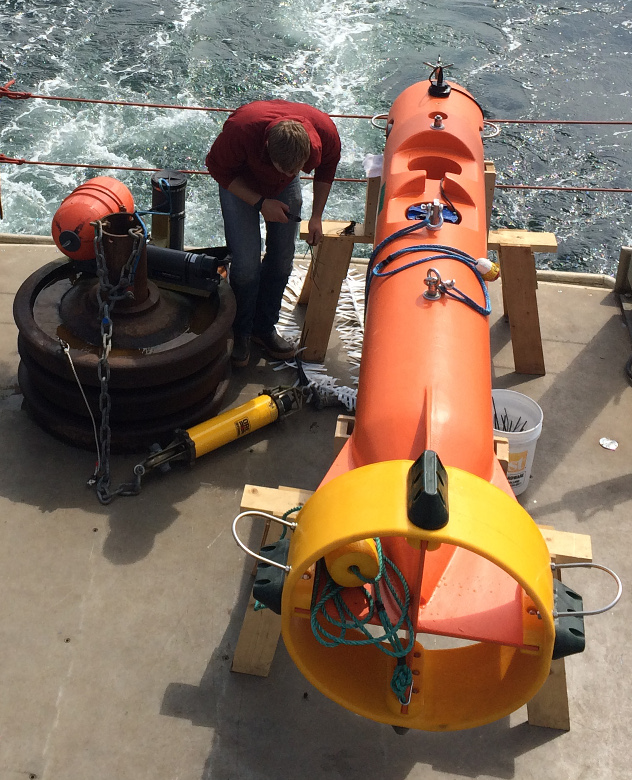
\includegraphics[width=2.6in]{SM_ondeck01}
  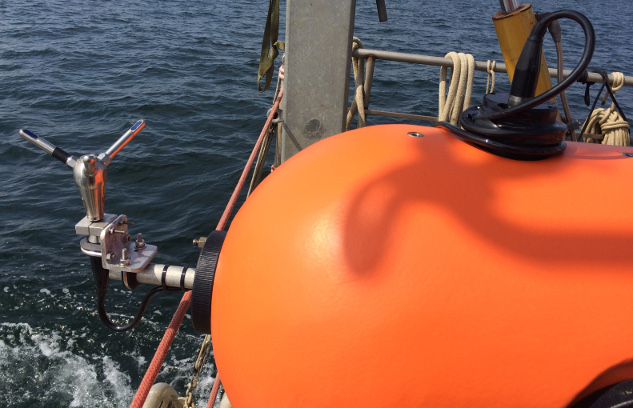
\includegraphics[width=2.6in]{SM_NoseMode01}
  \caption{Alex DeKlerk checks to ensure that the StableMoor buoy is properly fastened to its anchor; the RDI workhorse ADCP can be seen in the rear instrument bay (top). A bridle is draped across the top of the buoy for deployment and recovery, and a small marker buoy fastened to the tail aids in recovery.  A close-up of the StableMoor nose shows the ADV head and the top of its pressure case (bottom). }
  \label{fig:SM}
\end{figure}


\subsection{Principal-axes coordinate system and turbulence averaging}

Unless stated otherwise, vector quantities in this work are in a fixed `principal-axes' coordinate system that is aligned with the bi-directional tidal flow: positive $u$ is in the direction of ebb (310$\circ$ True), positive $w$ is vertically upward, and $v$ is the cross-stream component in a right-handed coordinate system. The full velocity vector, $\vec{\tilde{u}} = (\tilde{u}, \tilde{v}, \tilde{w})$, is separated into a mean and turbulent component as $\vec{\tilde{u}} = \vec{\bar{u}} + \vec{u}$, where---here and throughout this work---the over-bar denotes a 5 minute average.  All time series are linearly detrended and Hanning windowed prior to computing spectra to reduce spectral reddening. All spectra are computed as the variance preserving squared magnitude of the Fourier transform using standardized fast Fourier transform routines (i.e. $\int \spec{u}\mathrm{d}f = \overline{u^2}$).

\section{Methodology}
\label{sec:methods}

% The orientation matrix can be used to rotate all vector-quantities measured in the instrument frame (velocity, rotation rate, acceleration, etc.) into the earth's coordinate system. 
% The angular rate and linear acceleration signals can be used to estimate the ADV head-motion, $\uhead$, which can then be removed from the measured velocity, $\umeas$, to estimate the `motion corrected' velocity in the earth frame,
% Note that $\uhead$ is added to $\umeas$ because the measured velocity resulting from head motion is in the opposite direction of head motion itself (i.e., $\umeas = \ue - \uhead$).

The essential approach of this methodology is to estimate time-series of velocity on a compliant mooring by obtaining an independent estimate of ADV head motion and removing that motion from the measured signal. Nortek offers an ADV that is equipped with an IMU that measures the linear acceleration, rotational-motion, and orientation of the ADV pressure case (body). So long as the ADV head is rigidly connected to the ADV pressure case, it is possible to utilize the IMU motion signals to calculate the motion of the ADV head, and remove it from the measured velocity signal.  The ADV head motion, is calculated as the sum of rotational and translational motion, which are each estimated from the IMU's angular-rate, \AngRt, and acceleration, \Accel, signals as:
\begin{align}
  \uhead & = \urot + \uacc + \ulow \\
      & = \omatinv \cdot \AngRt^*(t)\times\l^* + \int \{\Accel(t)\}_{HP(f_{a})} \mathrm{d}t + \ulow
\end{align}
Here `$*$' superscripts denote quantities in the ADV's locale coordinate system, $\omatinv$ is the IMU orientation matrix that rotates vectors from the IMU to the earth reference frame, and $\l^*$ is the vector from the IMU to the ADV head. The notation $\{\Accel\}_{HP(f_a)}$ indicates that the IMU's accelerometer signal is high-pass filtered (in the earth's stationary reference frame) at a chosen filter-frequency, $f_a$. This is necessary because accelerometers have low-frequency noise, sometimes referred to as `bias-drift' \citeneeded{Accelerometer noise}. This noise is amplified by integration of the acceleration signal such that it contaminates the motion correction, especially at low-frequencies (Figure \ref{fig:stationary_noise}).  This issue means that low-frequency motion is not well resolved by the IMU, and so there is a residual low-frequency translational motion, $\ulow$, that needs to be considered when performing motion correction.

For the TTM we utilize $f_a = 0.0333 Hz$ (30 second period), and assume that $\ulow = 0$. For the StableMoor $f_a = 0.2 Hz$ (5 second period). The bottom-track velocity was  low-pass filtered at this frequency to provide an estimate of $\ulow$, and $\Accel$ was high-pass filtered at this frequency. We used 4-pole, bi-directional (zero-phase) Hanning filters for these filtering operations. 

% Do I need to say something about filtering out gravity here too?

% Bench-tests of the Microstrain IMU indicate that its accelerometers drift for frequencies $<10^{-2}$Hz (a minute or more, \cite{EgelandPhD2014}).  Therefore, in order to remove bias-drifts in $\vec{a}$ that--when integrated according to \eqref{eqn:uacc-def}--lead to large errors in $\uacc$ this document recommends using $f_a = 0.033$Hz (30seconds). 
% On the other hand, real motions at and below $f_a$ will not be accurately accounted for in $\uacc$, and will therefore persist as low-frequency motion contamination not corrected-for in the estimate of $\vec{u}$. 

% For moorings whose low-frequency motion is limited by the mooring line itself this is a reasonable approach.  
% Assuming that the displacement of the ADV head (from the mooring's neutral position) is likely to be  $< 20 \% $ of its distance from the bottom, then for ADVs deployed at 10m depth the speed of their low-frequency motion (i.e. below $ f_a = 0.03 $ Hz) will be $<0.07 \mathrm{m/s} $.  In other words, for a 10m mooring the choice of $f_a = 0.03$Hz allows for low-frequency motion contamination on the order of 7cm/s to persist.  This is a notable but relatively minor level of uncertainty in the context of the highly energetic flows that exist at tidal energy sites.

The choice of high-pass filter to be used to correct for low-frequency accelerometer noise issue depends on the application (e.g. deployment platform), and the turbulence level of the measurement environment. In particular, this involves a trade off between filtering-out this noise and not filtering measured motion (Figure \ref{fig:stationary_noise}). If an independent measure of low-frequency motion is available, it is possible to combine that signal with the IMU's high-frequency motion measurements to obtain a complete estimate of ADV motion. An example of this operation is presented in section \ref{sec:stablemoor_motion}. Lacking an independent measure of low-f motion, the user may instead choose to neglect the portion of the spectrum below the filter frequency, or demonstrate that platform motion at those frequencies is small compared to the measured signal based on other considerations. 

\begin{figure}
  \centering
  \label{fig:stationary_noise}
  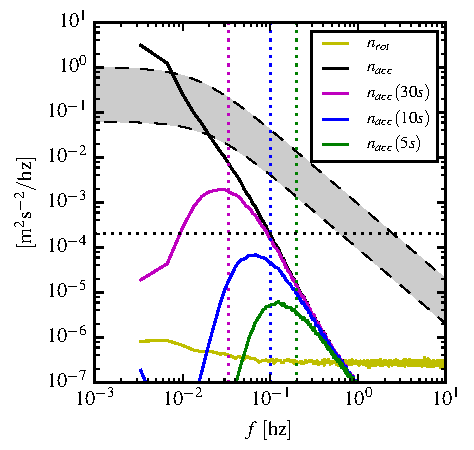
\includegraphics[width=\onewidth]{stationary_noise03}
  \caption{Spectra of $\urot$ (yellow) and $\uacc$ signals from the Microstrain IMU sitting on a motionless table. The $\uacc$ signals are unfiltered (black), and high-pass filtered at 30s (magenta), 10s (blue), 5s (green). Vertical dotted lines indicate the filter frequency. The black horizontal dotted line indicates the noise-level of a Nortek Vector ADV configured to measure $\pm$4m/s. The shaded region indicates the range of spectra presented herein (0.002 $< \tke <$ 0.03 $\mathrm{m^2/s^2}$, 1e-5 $< \epsilon <$ 5e-4 $\mathrm{W/kg}$).}
\end{figure}

With this estimate of ADV head motion it is straightforward to correct the measured velocity, $\umeas$, to estimate the velocity in the earth's inertial reference frame:
\begin{align}
  \label{eqn:u_mot_def}
  \ue(t) & = \umeas(t) + \uhead(t) &  .
\end{align}
Note here that the `+'-sign is correct because head motion, $\uhead$, induces a measured velocity in the opposite direction of the head motion itself ($\umeas = \ue - \uhead$).

\section{Results}

\begin{figure}[t]
  \centering
  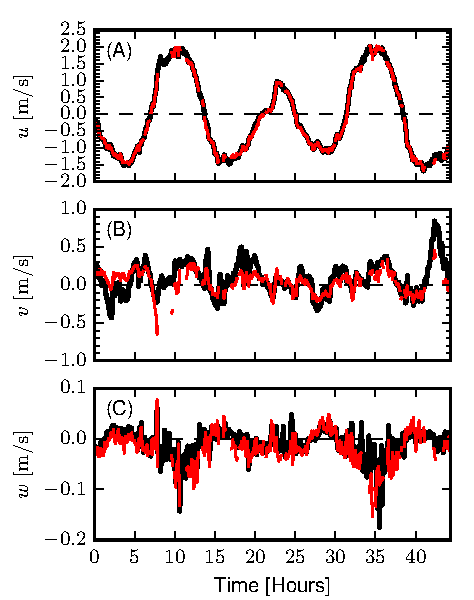
\includegraphics{TimeFig02}
  \caption{Time series of tidal velocity at Admiralty Head from TTM measurements (black), and an acoustic Doppler profiler (red). The profiler measurements--taken at the same depth as the ADV on the TTM---were contaminated by acoustic reflection from the strongback fin when it was inline with one of the profiler's beams. Note that the vertical scale on the three axes vary by more than an order of magnitude (the small ticks in A and B are equivalent to the ticks in C).}
  \label{fig:vel_time}
\end{figure}

\subsection{Mean velocity}

A comparison of mean velocity measured by an IMU-ADV mounted on a TTM, to that of an upward-looking acoustic Doppler profiler mounted on the TTM anchor is presented in Figure \ref{fig:vel_time}. This shows excellent agreement between the ADV and Doppler profiler measurements of velocity. The $u$, $v$ and $w$ components have a root-mean-square error of 0.05, 0.13 and 0.03 m/s, respectively. 
It is unclear why the $v$-component has a larger error than the others, but it may be due to side-lobe interference of an AWAC beam that was not captured by the screening methodology described in section \ref{sec:meas}. It is also possible that this discrepancy is due to incomplete motion correction that aliases into the mean signal.
%The $v$ component error is likely larger because the IMU's magnetometer provides a noisier estimate of heading than the accelerometers provide for vertical. 

The agreement between the magnitude and direction of these independent measurements indicates that the IMU provides an useful estimate of the ADV's orientation in the Earth's reference frame. This is a highly encouraging result considering most ADV manufacturers previously assumed these instruments would be stationary and therefore relied on slow-response orientation sensors.

\subsection{TTM Spectra}

\begin{figure*}[t]
  \centering
  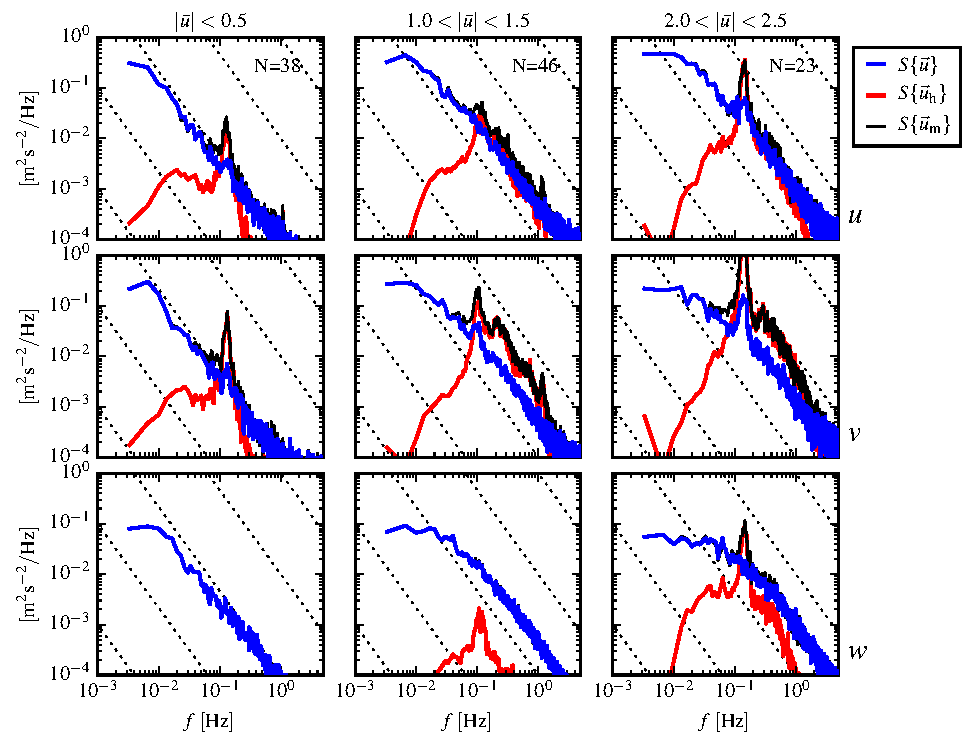
\includegraphics{SpecFig02_TTM02B-top}
  \caption{Turbulence spectra from the TTM for 3 ranges of mean stream-wise velocity (first column: $|u|< 0.5$ m/s, second column: $1 < |u| < 1.5$ m/s, third column: $2 < |u| < 2.5$ m/s). The rows are for each component of velocity (top: $u$, middle: $v$, bottom: $w$). The uncorrected spectra are in black and the corrected spectra are blue. The spectra of ADV head motion, $\uhead$, is red. Diagonal dotted-lines indicate a $f^{-5/3}$ slope. N is the number of spectral-ensembles in each column.}
  \label{fig:spec01}
\end{figure*}

As discussed in detail in the companion paper, the mooring motion of the TTM, $\spec{\uhead}$, has a peak at 0.1 to 0.2 Hz from swaying of the mooring that is most likely driven by eddy-shedding from the spherical buoy (Figure \ref{fig:spec01}, red lines). There is also broad-band motion that is associated with fluttering of the strongback fin around the mooring line. Both of these motions are especially energetic in the $v$-component spectra, because this is the direction in-which the TTM mooring system is most unstable. As would be expected from basic fluid-structure interaction theory the amplitude of these motions increases with increasing mean velocity \citeneeded{motion increasing with fluid velocity?}.

The mooring motion contaminates the uncorrected ADV-measurements of velocity, \spec{\umeas}, whenever the amplitude of the motion is similar to or greater than the amplitude of the turbulence. Fortunately, much of this motion can be removed using the IMU's motion signals as detailed in section \ref{sec:methods}. Lacking an independent measurement of turbulence velocity at this site, we interpret the agreement of these spectra with turbulence theory as evidence of the success of the method. In particular, for each mean-flow speed the spectra decay with a $f^{-5/3}$ slope and have equal amplitude across the velocity components. These results are consistent with Kolmogorov's (1941) theory of isotropic turbulence, and are consistent with other measurements of turbulence in energetic tidal channels from stationary platforms \citep[]{Kolmogorov1941c,Thomson++2010}.  \citeneeded{are there more citations here? Should I add a fig from the TTT?}

As successful as motion correction is, some of the motion contamination persists in $\spec{\ue}$. This is most notable in the $v$-component spectra at the highest flow speeds where a peak in $\spec{v}$ at 0.15 Hz is nearly an order of magnitude larger than a typical turbulence spectral fit to the other frequencies would indicate. This persistent motion contamination is evident to a lesser degree in the $u$-component spectra at the highest flow speed, and in the $v$-component spectra at lower flow speeds.  The $w$-component spectra appear to have no persistent motion contamination. This is largely because the amplitude of the motion in this direction is much lower than for the other two components. In fact, for these measurements, the $w$-component of mooring motion is so low that $w$-component motion correction is significant only at the highest flow speeds (i.e. motion correction removes the 0.15 Hz peak).

The amplitude of the persistent motion contamination peaks at 0.15 Hz are a factor of 5 to 10 times smaller than the amplitude of the ADV head motion itself. This suggests the Microstrain IMU's motion signals can be used to effectively correct for mooring motion at 0.15 Hz when the amplitude of that motion is less than 5 times the amplitude of the real turbulence spectrum.

% Does this belong in the discussion?
This reveals an ancillary benefit of the IMU measurements, which is that they can assist with identifying and accounting for persistent sources of motion contamination. For example, one of the most common uses of turbulence spectra is for the calculation of the turbulent kinetic energy dissipation rate, $\epsilon$, or for calculating the total turbulent kinetic energy, $\tke$. In particular, the regions of the spectrum where the motion is a factor of 3 to 5 larger than the measured signal can be excluded from a spectral fit. The fit can the be used to estimate $\tke$ and $\epsilon$. 
% Do we need to say something about the $v$-component time series being contaminated, but the $w$ and $u$ are relatively clean?

\subsection{StableMoor Spectra}

The spectra of the stablemoor motion has a broader peak with a maximum amplitude that is at approximately half the frequency of the TTM spectral peak (Figure \ref{fig:specSM01}). The motion of this platform also does not have high-frequency `sub-peaks' or other high-frequency broad-banded excitation. These characteristics of the motion are most-likely due to the more massive and hydro-dynamically streamlined nature of the platform. 

Like the TTM, the motion-corrected spectra from the StableMoor are consistent with turbulence theory and previous observations. Most importantly, there is an improvement in the quality of the motion corrected spectra compared to the TTM. In particular their does not appear to be significant persistent motion contamination peaks in these spectra. When the assumption that $\ulow=0$ is made, peaks and troughs are seen in the data, which suggests that the improvement in motion correction is largely the result of an accurate measurement of $\ulow$.

\begin{figure*}[t]
  \centering
  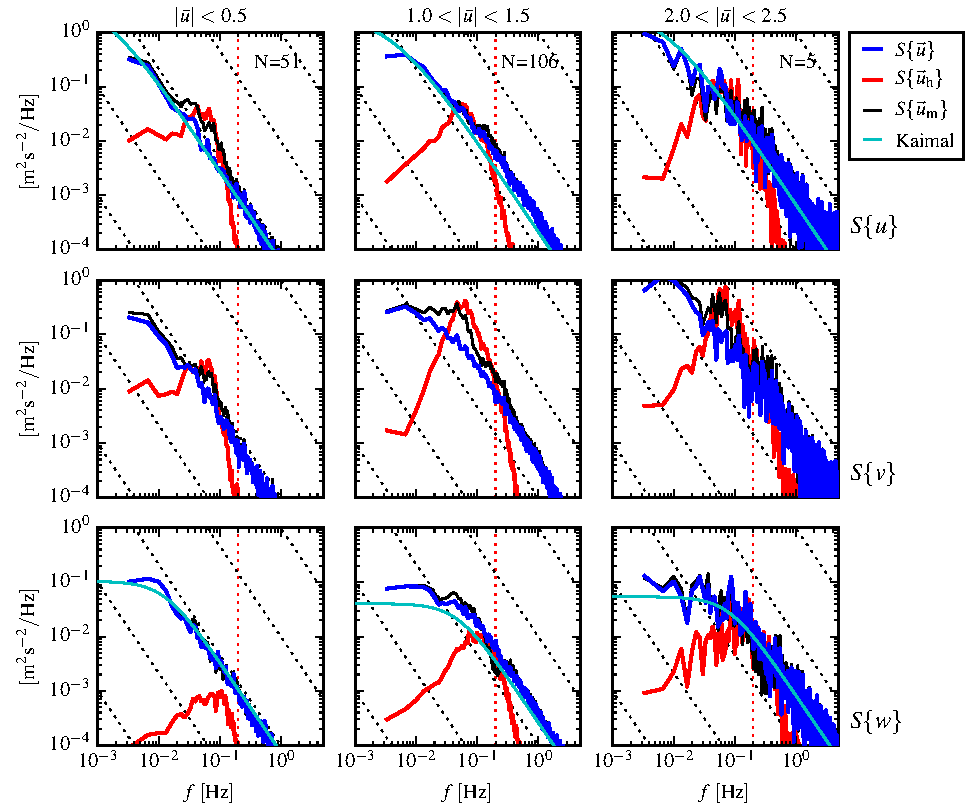
\includegraphics{SpecFig02_SMnose}
  \caption{Turbulence spectra from the StableMoor buoy. The axes-layout and annotations are identical to Figure \ref{fig:specSM01}.}
\end{figure*}

\section{Discussion}

For many applications, such as estimating the turbulence dissipation rate, or turbulent kinetic energy, estimating the spectra is an intermediate step...

- Compare the motion correction of SM to TTM: SM does better because it is more stable, and has a measurement of $u_\mathrm{low}$. Discuss spectral coherence of $u_\mathrm{BT}$ with IMU, i.e. Figure \ref{fig:SM_coh}. This is important because it shows the low-$f$ limit of the IMU measured motion.

- $\uhead$ provides a justification, and a screening criteria(?), for removing portions of the signal.
- Can estimate $\epsilon$, tke with fits that exclude contaminated portions of the spectra.
- Can remove up to 10x signal motion
- Discuss the time-domain method vs. spectral (cross-coherence) methods, and the need for phase information.

\begin{figure}[t]
  \centering
  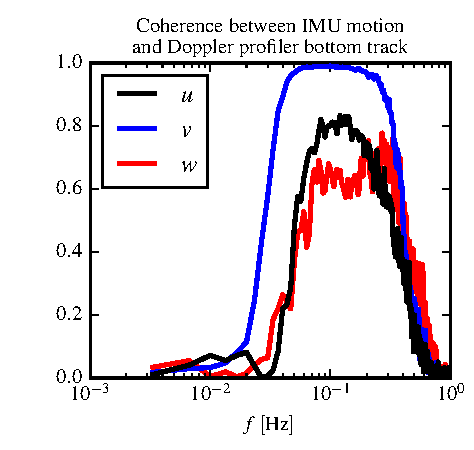
\includegraphics{BT_IMU_Coherence02}
  \caption{Coherence between stablemoor IMU measured motion and bottom track velocity.}
  \label{fig:SM_coh}
\end{figure}

\section{Conclusion}


%\subsubsection{Uncertainty in spectra}

%\subsection{Turbulence energy dissipation rate}

%%%%%%%%%%%%%%%%%
%ACKNOWLEDGMENTS
%%%%%%%%%%%%%%%%%

\acknowledgments


\clearpage %REMOVE_FOR_SUBMIT

%%%%%%%%%%%%%%%%%
%APPENDIXES
%%%%%%%%%%%%%%%%%
\appendix


\appendixtitle{Coordinate Systems}

\def\Amat\ensuremath{\mathbf{A}}

\subsection{IMU uncertainty}\label{apdx:imu-uncertainty}

\subsection{Measurement frames}\label{apdx:coord-sys:meas}\label{apdx:coord-sys}

\def\a{\ensuremath{\mathrm{a}}}
\def\b{\ensuremath{\mathrm{b}}}
\def\lab{\ensuremath{l_\b^\a}}
\def\xa{\ensuremath{\vec{r}^\a}}
\def\xb{\ensuremath{\vec{r}^\b}}
\def\Rba{\ensuremath{\mathbf{R}^\a_\b}}

Tracking coordinate systems (`reference frames', or simply `frames') is critical to accurately correcting for platform motion of ADV measurements. In general, two three-dimensional, orthogonal, right-handed coordinate systems `a' and `b' are related by the equation:
\begin{align*}
  \xb &= \Rba \cdot (\xa - \lab) & .
\end{align*}
The vectors $\xa$ and $\xb$ point to the same point in space, but in the two distinct coordinate systems.  Superscripts denote the coordinate system that the quantity is measured in and $\cdot$ indicates standard matrix multiplication.  The vector $\lab$ is the `translation vector' that specifies the origin of coordinate system `b' in the `a' frame, and $\mathbf{R}^\mathrm{a}_\mathrm{b}$ is the `orientation matrix' of `b' in `a'. Note that the equation that maps vectors - as opposed to points in space - from one frame to the other does not include $\lab$:
\begin{align}
  \vec{u}^\mathrm{b} & = \Rba \cdot \vec{u}^\mathrm{a}
\end{align}
Also note that for the orthogonal, right-handed coordinate systems considered here the inverse rotation matrix is simply the transpose, $\mathbf{R}^{\mathrm{b}}_{\mathrm{a}}  = (\Rba)^{-1} = (\Rba)^\mathrm{T} $, and the determinant of the rotation matrix is 1, $\mathrm{det}(\Rba ) = 1$.
The coordinate systems for doing so can be broken into two categories: 1) the `inertial' or `stationary' ones into which it is the goal to transform the measurements, and 2) the moving coordinate systems in which sensors make measurements. 

The purpose of this appendix is to clearly document and define the relationships between all of the coordinate systems necessary for quantifying turbulence using moored ADVs.  This appendix starts with general definitions of coordinate systems and the relationships between them (\ref{apdx:coord-sys:math}), then details the stationary and measurement frames used herein (\ref{apdx:coord-sys:stat} and \ref{apdx:coord-sys:meas}, respectively).

\begin{enumerate}
\item the earth reference frame is the inertial coordinate system in
which it is desirable to have measurements of turbulence velocity
\item the IMU reference frame is the reference frame in which that
sensor measures platform motion
\item the ADV-head reference frame is the reference frame in which the
velocity measurements are obtained.
\end{enumerate}

In addition to measuring platform motion the Microstrain IMU provides
an estimate of the orientation of its coordinate system in the earth's
reference frame. Provided that the position and orientation of the
ADV-head is known and fixed in the IMU frame (i.e. they are rigidly
connected), it is possible to estimate the motion of the ADV-head in
the earth reference frame.




\subsection{Defining coordinate systems}\label{apdx:coord-sys:math}


\subsection{The earth frame}
The earth coordinate system is the coordinate system in-which the orientation of the ADV is measured (see \ref{apdx:coord-sys:imu}), and is the coordinate system in-which motion correction is most easily calculated and discussed (section \ref{sec:proc:motion}).  This work utilizes `e' superscripts to denote an `ENU' earth coordinate system with basis vectors,
\begin{itemize}
\item[$\hat{x}\earth$:] East,
\item[$\hat{y}\earth$:] North, and
\item[$\hat{z}\earth$:] Up.
\end{itemize}

\begin{figure}
  \centering
  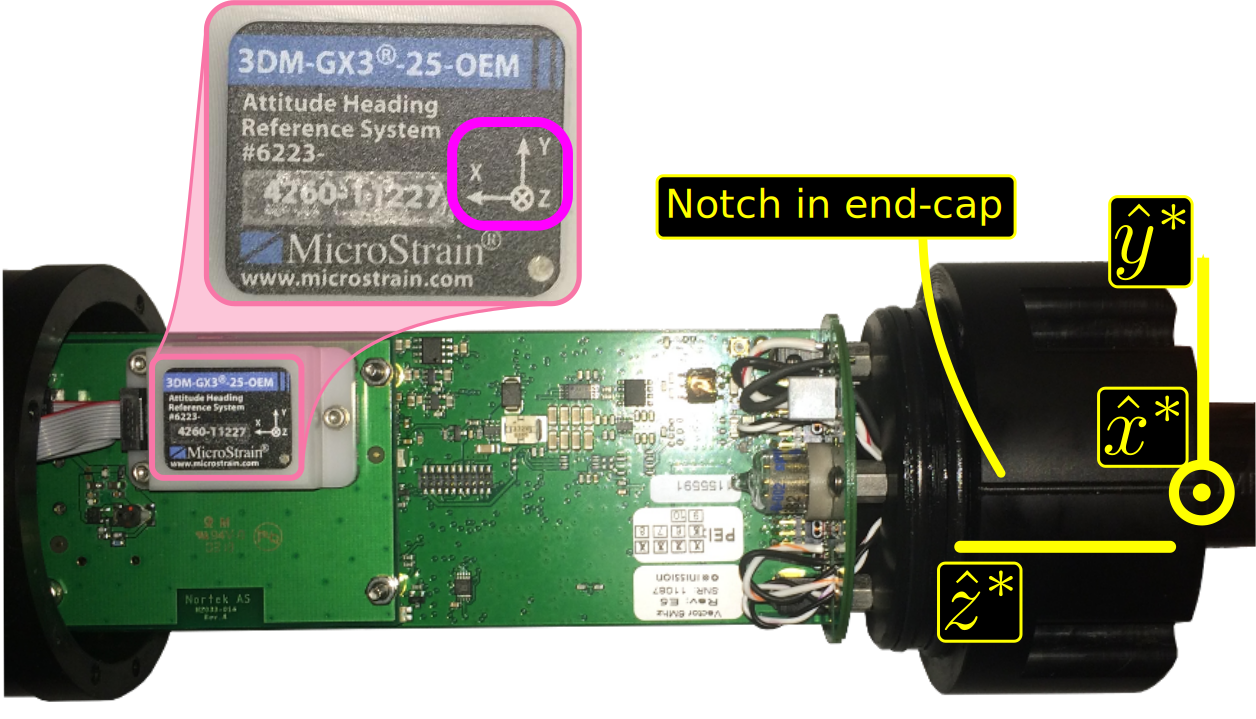
\includegraphics[width=\onewidth]{IMU_Diagram04}
  \caption{The circuit-board and pressure-case end-cap of a Nortek Vector equipped with a Microstrain IMU.  The ADV-body coordinate system (yellow) is depicted on the right. The notch in the end-cap defines the $\hat{x}^*$ direction (out of the page), and the $\hat{z}^*$ direction points back along the pressure case axis. A zoom-in on the Microstrain chip highlights its coordinate system (magenta) relative to the body. }
  \label{fig:imu_orient}
\end{figure}

To combine signals from an IMU with those of an ADV to perform motion correction the coordinate systems in which each of the measurements are made must be carefully accounted for. 

For the Nortek Vector instruments that were used for this work the `ADV-body' coordinate system is defined as being centered on the cylinder-body axis at the point where the head-cable meets its end-cap.  The basis vectors of this coordinate system are defined as (Figures \ref{fig:imu_orient} and \ref{fig:adv-coord-sys}B):
\begin{itemize}
\item[$\hat{x}^*$:] points from the center of the `head' end-cap toward the notch in that end-cap,
\item[$\hat{y}^*$:] is defined by the right-hand-rule based on the other two basis vectors, and
\item[$\hat{z}^*$:] points from the `head' end-cap toward the `battery' end-cap along the body-cylinder (pressure case) axis.
\end{itemize}

\subsubsection{The ADV head}

In order to transform measured velocities into a meaningful reference frame (and to perform motion correction) the orientation (and position) of the ADV head in terms of the body coordinate system must be known. To facilitate this the orientation matrix of the ADV head, $\rmat$, and translation vector\footnote{The position of the ADV-head origin (transmit transducer) in the body coordinate system.}, $\bhv$, are defined according to,
\begin{align}
  \label{eqn:coord_sys}
  \vec{x}^\mathrm{head} &= \rmat \cdot (\vec{x}^* - \bhv) & ,
\end{align}
where $\vec{x}^\mathrm{head}$ and $\vec{x}^*$ are the same point in the head and body coordinate systems, respectively. Combined with the math notes in the previous section, the velocity vectors in the head frame can be transformed into the body frame by,
\begin{align}
  \label{eqn:coord_sys2}
  \vec{u}^* &=  \rmat^\mathrm{T} \cdot \vec{u}^\mathrm{head} & .
\end{align}

For Nortek Vectors, the coordinate system of the ADV head is centered on the transmit transducer face, and the coordinate-directions are defined by (Figure \ref{fig:adv-coord-sys}B, \cite{vector_manual2005}):
\begin{itemize}
\item[$\hat{x}^\mathrm{head}$:] the direction of one of the transducer `receive' arms (marked with tape or paint)
\item[$\hat{y}^\mathrm{head}$:] is defined by the right-hand-rule based on the other two basis vectors, and
\item[$\hat{z}^\mathrm{head}$:] is into the transducer face.
\end{itemize}

For fixed-head Nortek Vector ADVs, the body-frame and head-frame have parallel coordinate systems ($\rmat$ is the identity matrix), and the `head-frame' is translated 21cm along the $z$-axis.  That is, $\bhv = (0, 0, -0.21)$m \cite[]{vector_manual2005}.  

For cable-head ADVs, the position and orientation of the ADV head is arbitrary.  This means that when preparing to make measurements using cable-head ADVs, {\bf the orientation and position of the ADV head must be accurately recorded} in order to allow the ADV measurements to be transformed into the body frame during post-processing. For the example in Figure \ref{fig:adv-coord-sys}A, $\bhv = (254,64,-165)\unit{mm}$, and
\begin{align*}
  \rmat &= \left (
    \begin{array}{ccc}
      0 & 0 & -1 \\
      0 & -1 & 0 \\
      -1 & 0 & 0
    \end{array}
    \right ) & .
\end{align*}
In general $\rmat$ will not necessarily be symmetric nor will it have so many zero-elements (i.e. these characteristics are specific to the head-body alignment of the example).


\begin{figure}
  \centering
  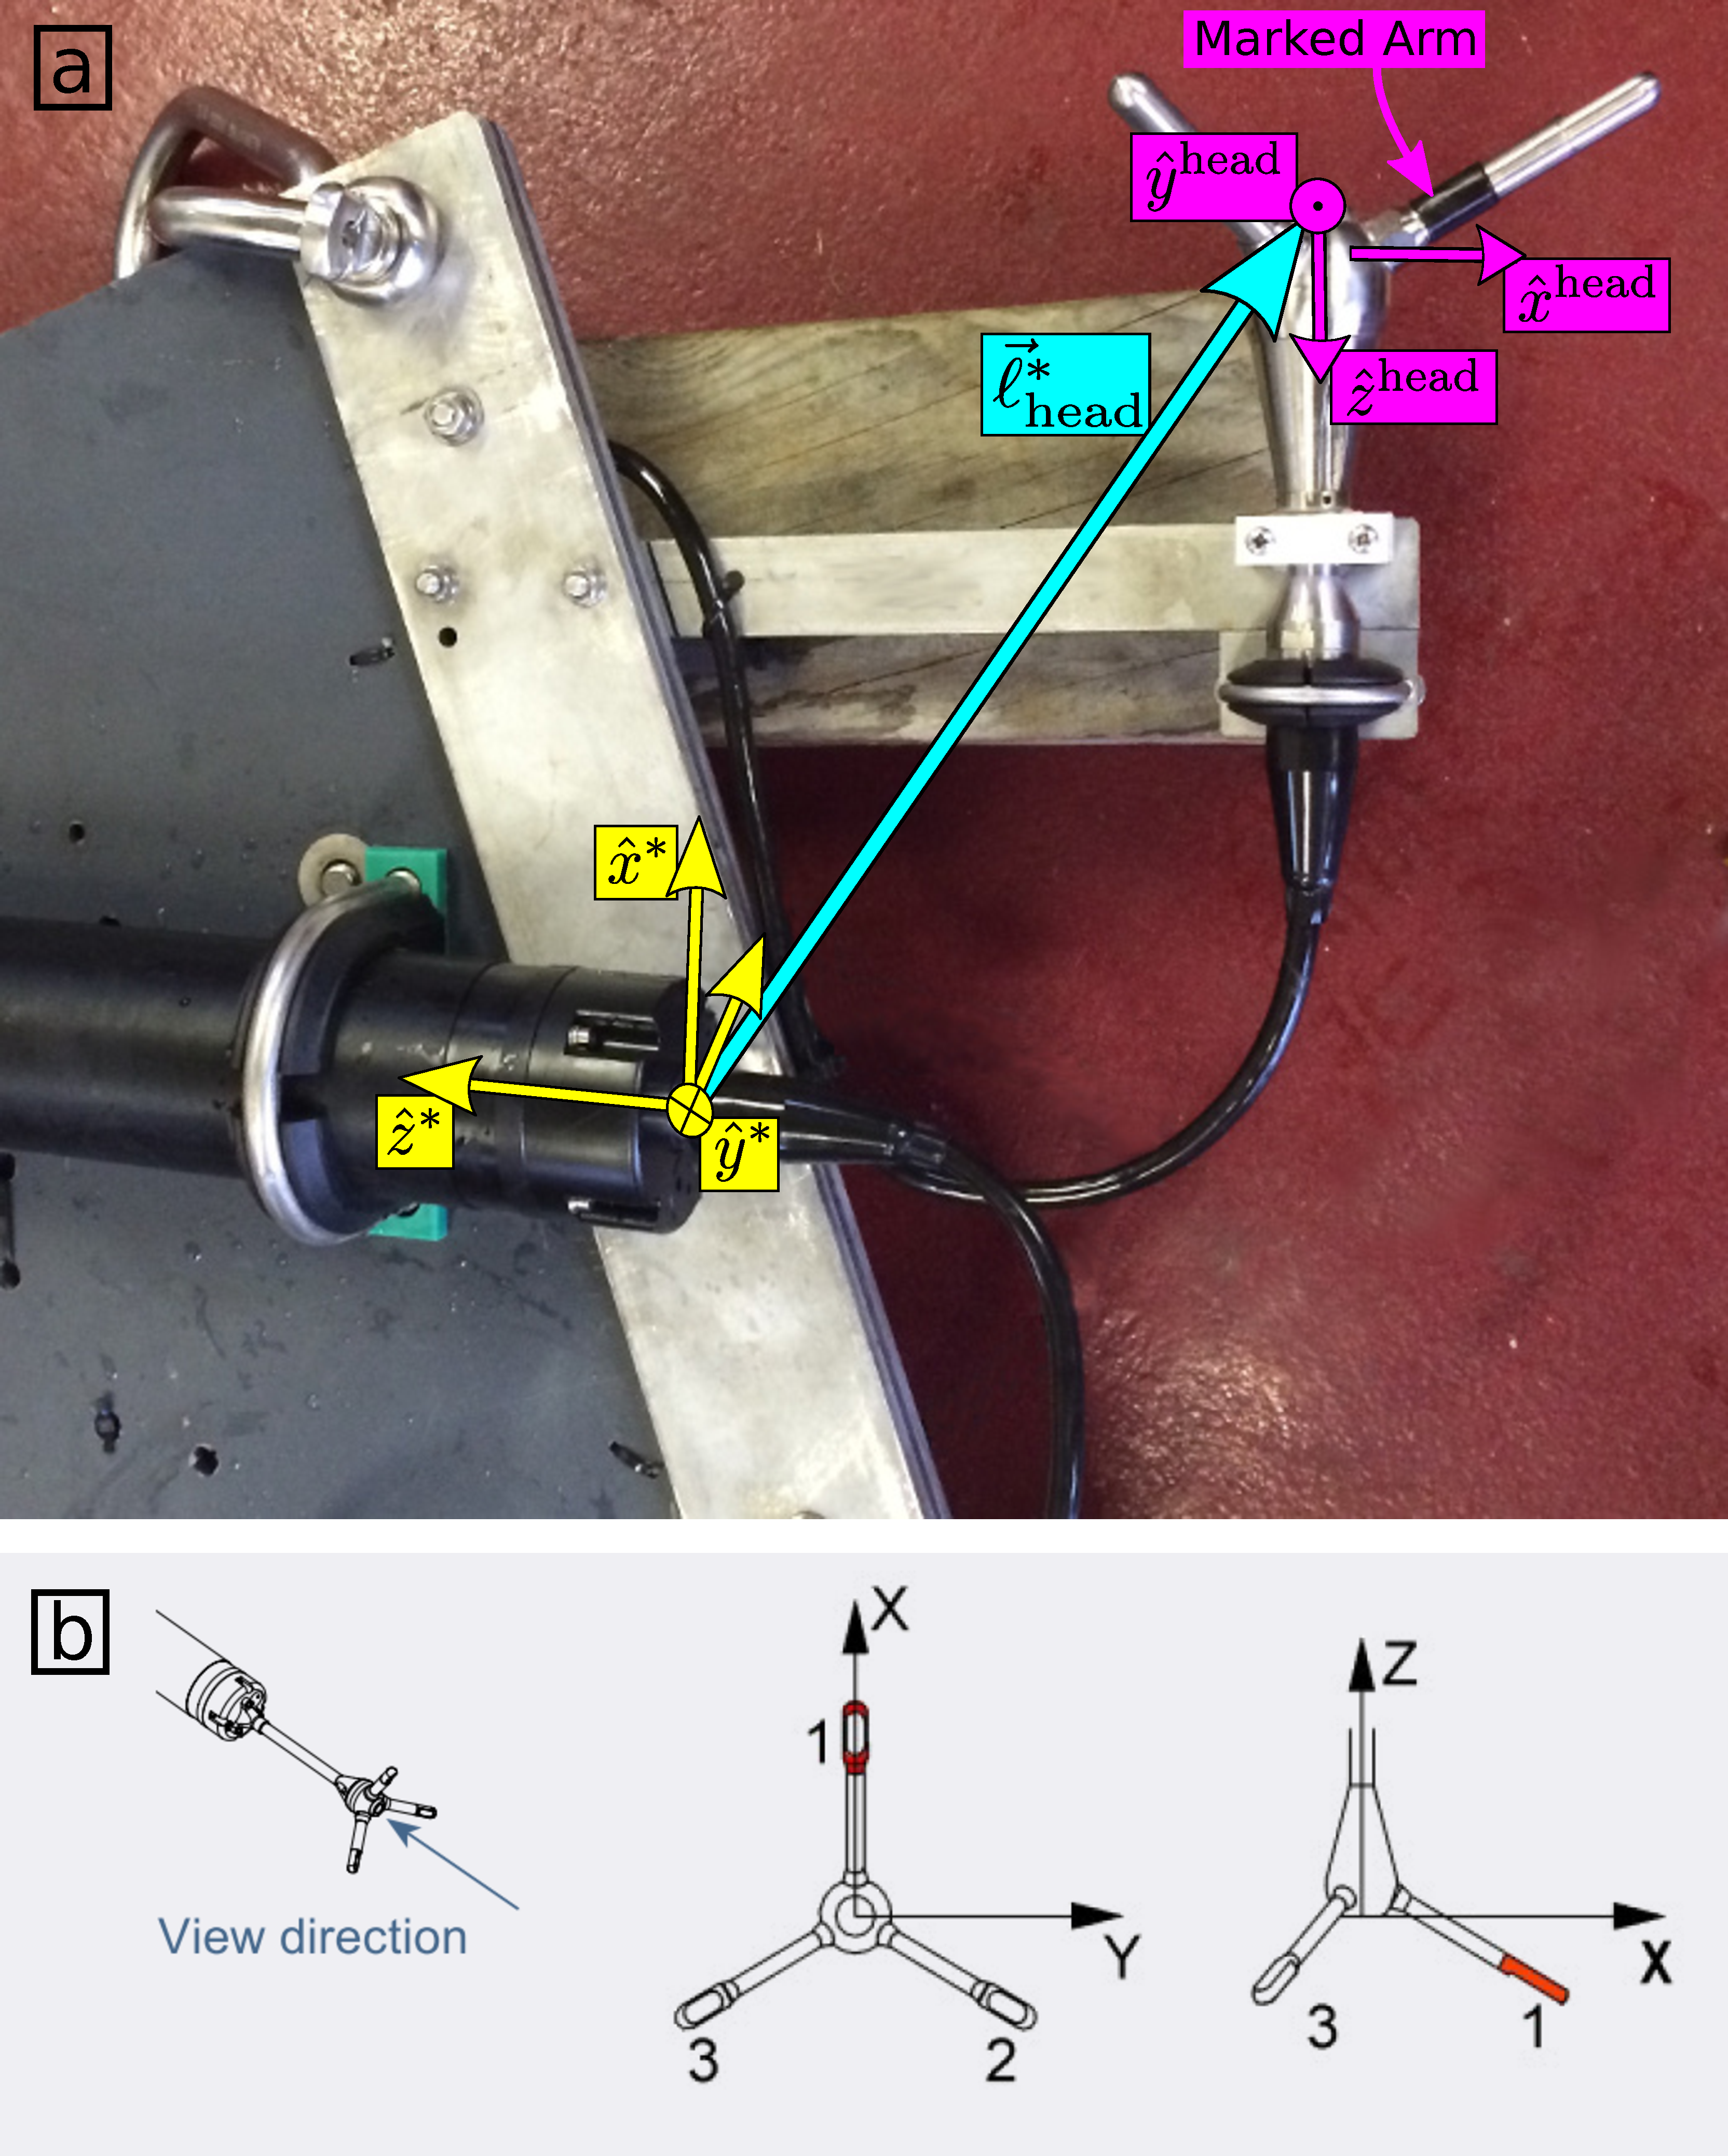
\includegraphics[width=\onewidth]{ADV_coord_sys}
  \caption{Coordinate systems of the ADV body and head. A) A strongback with an ADV rests on a block of wood. Coordinate systems of the ADV head (magenta) and body (yellow) are shown. The $\hat{x}^\mathrm{head}$-direction is known by the black-band around the transducer arm, and the $\hat{x}^*$ direction is marked by a notch on the end-cap (indiscernible in the image). The cyan arrow indicates the body-to-head vector, $\bhv$.  The perspective slightly distorts the fact that  $\hat{x}^\mathrm{head} \parallel -\hat{z}^* $, $\hat{y}^\mathrm{head} \parallel -\hat{y}^* $, and $\hat{z}^\mathrm{head} \parallel -\hat{x}^* $.  B) Coordinate system of the ADV head as defined in the Nortek Vector manual \cite[]{vector_manual2005}. }
  \label{fig:adv-coord-sys}
\end{figure}

\subsubsection{The IMU coordinate system}\label{apdx:coord-sys:imu}

Like the ADV head, the coordinate system in which the IMU measurements are made must be clearly defined and documented. In general, the IMU frame is related to the body coordinate system by,
\begin{align*}
  \vec{x}^\mathrm{imu} &= \mathbf{A}  \cdot (\vec{x}^* - \ihv) & \qquad .
\end{align*}

For the Microstrain 3DM-GX3-25 (IMU) as it is integrated into the Nortek Vector (Figure \ref{fig:imu_orient}), $\ihv = (0.006, 0.006, 0.150)$m and,
\begin{align*}
  \mathbf{A} &=
  \left (
    \begin{array}{ccc}
      0 & 0 & 1 \\
      0 & 1 & 0 \\
      -1 & 0 & 0
    \end{array}
  \right ) & .
\end{align*}


{\bf The orientation matrix}
\def\omatr{\ensuremath{\mathrm{\mathbf{R_\mathrm{imu}}}}}

In order to use the orientation matrix to rotate velocity measurements into an earth-fixed coordinate system it is important to understand how the orientation matrix is defined. The Microstrain IMU outputs an orientation matrix, \omatr, such that:
\begin{align*}
  \vec{u}^\mathrm{imu} & = \omatr \cdot \vec{u}^\mathrm{NED} & .
\end{align*}
Where $\vec{u}^\mathrm{imu}$ and $\vec{u}^\mathrm{NED}$ are vectors in the IMU's local coordinate system and a `north-east-down' (NED) earth-fixed coordinate system, respectively \cite[]{Microstrain2012a}.  
However, this NED earth coordinate system is different from the ENU earth coordinate system used here (and typically used by Nortek \cite[]{nortek_sys_int_manual2011}).  That is,
\begin{align*}
  \vec{u} &= \mathbf{B} \cdot \vec{u}^\mathrm{NED} & ,
\end{align*}
where,
\begin{align*}
  \mathbf{B} & = 
  \left (
    \begin{array}{ccc}
      0 & 1 & 0 \\
      1 & 0 & 0 \\
      0 & 0 & -1
    \end{array}
  \right ) \qquad .
\end{align*}
From this, and the above discussion of the orientation of the IMU in the ADV, it is simple to show that the orientation matrix of the ADV body in a ENU earth frame is,
\begin{align*}
  \omat &= \mathbf{A} \cdot \omatr \cdot \mathbf{B} & ,
\end{align*}
%The \dolfyn\ software package makes this transformation when reading the orientation matrix from Nortek Vector `{\it .vec}' files (i.e. the `orientmat' attribute in the data object returned by \dolfyn .io.read\_nortek is \omat, not \omatr ).  This way vectors in the body frame can be rotated into the ENU earth frame by,
 % \begin{align*}
 %   \vec{u} & = \omatinv \cdot \vec{u}^* & .
 % \end{align*}


%%%%%%%%%%%%%%%%%
%REFERENCES
%%%%%%%%%%%%%%%%%

\bibliographystyle{ametsoc2014}
\bibliography{all}


\end{document}





